% ---------------------------------------------------------------
%  EnergyTech / معهد الطاقة  --  Chapter 04
%  Questions + answer choices + QR codes.
%  Scale diagrams are TikZ; the two labelled instrument photographs
%  live in figures/.
%  Compile with pdflatex (needs the 'qrcode' package).
% ---------------------------------------------------------------
\documentclass[11pt]{article}
\usepackage[a4paper,margin=1.8cm]{geometry}
\usepackage{amsmath,amssymb}
\usepackage{enumitem}
\usepackage{qrcode}
\usepackage{graphicx}
\usepackage{xcolor}
\usepackage[hidelinks]{hyperref}
\usepackage{multicol}

\setlength{\parindent}{0pt}
\setlength{\columnsep}{20pt}
\graphicspath{{figures/}}

\newcommand{\incfig}[2]{%
  \par\smallskip\begingroup\centering
  \ifdim #1pt>\linewidth\relax
    \includegraphics[width=\linewidth]{#2}%
  \else
    \includegraphics[width=#1pt]{#2}%
  \fi
  \par\endgroup\smallskip}

\newenvironment{Qbox}[2]{%
  \par\medskip\noindent\begin{minipage}{\linewidth}%
  \hrule\medskip%
  \textbf{Q#1)}\hfill\textbf{\underline{#2}}\par\smallskip%
}{\par\end{minipage}\par\medskip}

\newlist{choices}{enumerate}{1}
\setlist[choices]{label=\Alph*), itemsep=1pt, topsep=3pt, parsep=0pt, leftmargin=2em}
% ---------------------------------------------------------------

% ================= figure styles =================
\usepackage{tikz}
\usetikzlibrary{arrows.meta,calc,shadings}

\definecolor{figline}{RGB}{30,30,30}
\definecolor{figpanel}{RGB}{243,243,243}
\definecolor{figmark}{RGB}{63,63,160}
\definecolor{figbody}{RGB}{232,234,238}
\definecolor{figthimble}{RGB}{205,210,219}

\tikzset{
  sc/.style   ={draw=figline, line width=0.5pt, line cap=butt},
  scb/.style  ={draw=figline, line width=0.8pt},
  lab/.style  ={font=\small\bfseries, inner sep=1pt},
  labs/.style ={font=\scriptsize\bfseries, inner sep=1pt},
  ptr/.style ={draw=figmark, line width=1pt, -{Latex[length=4pt,width=3.5pt]}},
}

\newcommand{\figbox}[1]{%
  \par\smallskip\begingroup\centering
  \sbox0{#1}%
  \ifdim\wd0>\linewidth \resizebox{\linewidth}{!}{\usebox0}\else\usebox0\fi
  \par\endgroup\smallskip}

% ---- figure definitions ----
\newcommand{\figQBZ}{%
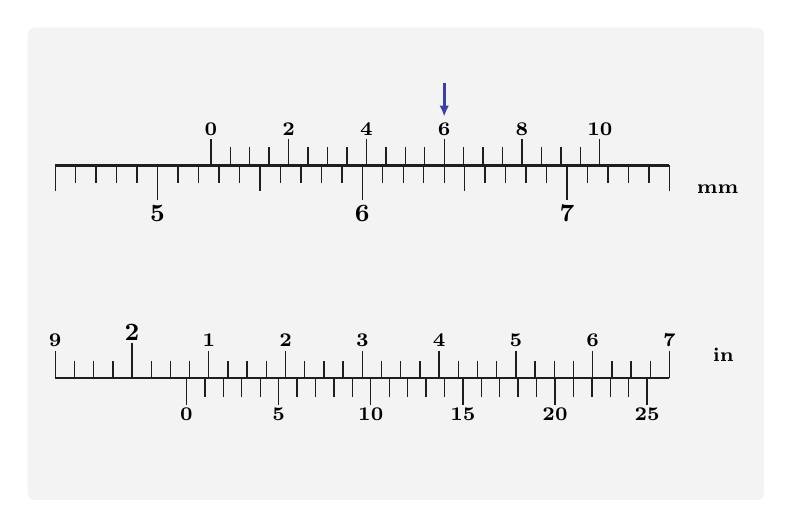
\begin{tikzpicture}[scale=1]
  \fill[figpanel,rounded corners=2pt] (-0.35,-1.55) rectangle (9,4.45);
  \begin{scope}[yshift=2.70cm]
  \draw[scb] (0,0) -- (7.8,0);
  \draw[sc] (0,0) -- (0,-0.32);
  \draw[sc] (0.26,0) -- (0.26,-0.22);
  \draw[sc] (0.52,0) -- (0.52,-0.22);
  \draw[sc] (0.78,0) -- (0.78,-0.22);
  \draw[sc] (1.04,0) -- (1.04,-0.22);
  \draw[sc] (1.3,0) -- (1.3,-0.44);
  \node[lab,below] at (1.3,-0.46) {5};
  \draw[sc] (1.56,0) -- (1.56,-0.22);
  \draw[sc] (1.82,0) -- (1.82,-0.22);
  \draw[sc] (2.08,0) -- (2.08,-0.22);
  \draw[sc] (2.34,0) -- (2.34,-0.22);
  \draw[sc] (2.6,0) -- (2.6,-0.32);
  \draw[sc] (2.86,0) -- (2.86,-0.22);
  \draw[sc] (3.12,0) -- (3.12,-0.22);
  \draw[sc] (3.38,0) -- (3.38,-0.22);
  \draw[sc] (3.64,0) -- (3.64,-0.22);
  \draw[sc] (3.9,0) -- (3.9,-0.44);
  \node[lab,below] at (3.9,-0.46) {6};
  \draw[sc] (4.16,0) -- (4.16,-0.22);
  \draw[sc] (4.42,0) -- (4.42,-0.22);
  \draw[sc] (4.68,0) -- (4.68,-0.22);
  \draw[sc] (4.94,0) -- (4.94,-0.22);
  \draw[sc] (5.2,0) -- (5.2,-0.32);
  \draw[sc] (5.46,0) -- (5.46,-0.22);
  \draw[sc] (5.72,0) -- (5.72,-0.22);
  \draw[sc] (5.98,0) -- (5.98,-0.22);
  \draw[sc] (6.24,0) -- (6.24,-0.22);
  \draw[sc] (6.5,0) -- (6.5,-0.44);
  \node[lab,below] at (6.5,-0.46) {7};
  \draw[sc] (6.76,0) -- (6.76,-0.22);
  \draw[sc] (7.02,0) -- (7.02,-0.22);
  \draw[sc] (7.28,0) -- (7.28,-0.22);
  \draw[sc] (7.54,0) -- (7.54,-0.22);
  \draw[sc] (7.8,0) -- (7.8,-0.32);
  \draw[sc] (1.976,0) -- (1.976,0.34);
  \node[labs,above] at (1.976,0.34) {0};
  \draw[sc] (2.223,0) -- (2.223,0.24);
  \draw[sc] (2.47,0) -- (2.47,0.24);
  \draw[sc] (2.717,0) -- (2.717,0.24);
  \draw[sc] (2.964,0) -- (2.964,0.34);
  \node[labs,above] at (2.964,0.34) {2};
  \draw[sc] (3.211,0) -- (3.211,0.24);
  \draw[sc] (3.458,0) -- (3.458,0.24);
  \draw[sc] (3.705,0) -- (3.705,0.24);
  \draw[sc] (3.952,0) -- (3.952,0.34);
  \node[labs,above] at (3.952,0.34) {4};
  \draw[sc] (4.199,0) -- (4.199,0.24);
  \draw[sc] (4.446,0) -- (4.446,0.24);
  \draw[sc] (4.693,0) -- (4.693,0.24);
  \draw[sc] (4.94,0) -- (4.94,0.34);
  \node[labs,above] at (4.94,0.34) {6};
  \draw[sc] (5.187,0) -- (5.187,0.24);
  \draw[sc] (5.434,0) -- (5.434,0.24);
  \draw[sc] (5.681,0) -- (5.681,0.24);
  \draw[sc] (5.928,0) -- (5.928,0.34);
  \node[labs,above] at (5.928,0.34) {8};
  \draw[sc] (6.175,0) -- (6.175,0.24);
  \draw[sc] (6.422,0) -- (6.422,0.24);
  \draw[sc] (6.669,0) -- (6.669,0.24);
  \draw[sc] (6.916,0) -- (6.916,0.34);
  \node[labs,above] at (6.916,0.34) {10};
  \draw[ptr] (4.94,1.05) -- (4.94,0.62);
  \node[labs,left] at (8.72,-0.30) {mm};
  \end{scope}
  \begin{scope}[yshift=0cm]
  \draw[scb] (0,0) -- (7.8,0);
  \draw[sc] (0,0) -- (0,0.34);
  \node[labs,above] at (0,0.36) {9};
  \draw[sc] (0.2438,0) -- (0.2438,0.22);
  \draw[sc] (0.4875,0) -- (0.4875,0.22);
  \draw[sc] (0.7313,0) -- (0.7313,0.22);
  \draw[sc] (0.975,0) -- (0.975,0.44);
  \node[lab,above] at (0.975,0.44) {2};
  \draw[sc] (1.2188,0) -- (1.2188,0.22);
  \draw[sc] (1.4625,0) -- (1.4625,0.22);
  \draw[sc] (1.7063,0) -- (1.7063,0.22);
  \draw[sc] (1.95,0) -- (1.95,0.34);
  \node[labs,above] at (1.95,0.36) {1};
  \draw[sc] (2.1938,0) -- (2.1938,0.22);
  \draw[sc] (2.4375,0) -- (2.4375,0.22);
  \draw[sc] (2.6813,0) -- (2.6813,0.22);
  \draw[sc] (2.925,0) -- (2.925,0.34);
  \node[labs,above] at (2.925,0.36) {2};
  \draw[sc] (3.1688,0) -- (3.1688,0.22);
  \draw[sc] (3.4125,0) -- (3.4125,0.22);
  \draw[sc] (3.6562,0) -- (3.6562,0.22);
  \draw[sc] (3.9,0) -- (3.9,0.34);
  \node[labs,above] at (3.9,0.36) {3};
  \draw[sc] (4.1438,0) -- (4.1438,0.22);
  \draw[sc] (4.3875,0) -- (4.3875,0.22);
  \draw[sc] (4.6313,0) -- (4.6313,0.22);
  \draw[sc] (4.875,0) -- (4.875,0.34);
  \node[labs,above] at (4.875,0.36) {4};
  \draw[sc] (5.1188,0) -- (5.1188,0.22);
  \draw[sc] (5.3625,0) -- (5.3625,0.22);
  \draw[sc] (5.6063,0) -- (5.6063,0.22);
  \draw[sc] (5.85,0) -- (5.85,0.34);
  \node[labs,above] at (5.85,0.36) {5};
  \draw[sc] (6.0938,0) -- (6.0938,0.22);
  \draw[sc] (6.3375,0) -- (6.3375,0.22);
  \draw[sc] (6.5813,0) -- (6.5813,0.22);
  \draw[sc] (6.825,0) -- (6.825,0.34);
  \node[labs,above] at (6.825,0.36) {6};
  \draw[sc] (7.0688,0) -- (7.0688,0.22);
  \draw[sc] (7.3125,0) -- (7.3125,0.22);
  \draw[sc] (7.5563,0) -- (7.5563,0.22);
  \draw[sc] (7.8,0) -- (7.8,0.34);
  \node[labs,above] at (7.8,0.36) {7};
  \draw[sc] (1.6673,0) -- (1.6673,-0.34);
  \node[labs,below] at (1.6673,-0.34) {0};
  \draw[sc] (1.9013,0) -- (1.9013,-0.24);
  \draw[sc] (2.1353,0) -- (2.1353,-0.24);
  \draw[sc] (2.3693,0) -- (2.3693,-0.24);
  \draw[sc] (2.6033,0) -- (2.6033,-0.24);
  \draw[sc] (2.8373,0) -- (2.8373,-0.34);
  \node[labs,below] at (2.8373,-0.34) {5};
  \draw[sc] (3.0713,0) -- (3.0713,-0.24);
  \draw[sc] (3.3053,0) -- (3.3053,-0.24);
  \draw[sc] (3.5393,0) -- (3.5393,-0.24);
  \draw[sc] (3.7733,0) -- (3.7733,-0.24);
  \draw[sc] (4.0072,0) -- (4.0072,-0.34);
  \node[labs,below] at (4.0072,-0.34) {10};
  \draw[sc] (4.2413,0) -- (4.2413,-0.24);
  \draw[sc] (4.4753,0) -- (4.4753,-0.24);
  \draw[sc] (4.7093,0) -- (4.7093,-0.24);
  \draw[sc] (4.9433,0) -- (4.9433,-0.24);
  \draw[sc] (5.1773,0) -- (5.1773,-0.34);
  \node[labs,below] at (5.1773,-0.34) {15};
  \draw[sc] (5.4113,0) -- (5.4113,-0.24);
  \draw[sc] (5.6453,0) -- (5.6453,-0.24);
  \draw[sc] (5.8793,0) -- (5.8793,-0.24);
  \draw[sc] (6.1133,0) -- (6.1133,-0.24);
  \draw[sc] (6.3473,0) -- (6.3473,-0.34);
  \node[labs,below] at (6.3473,-0.34) {20};
  \draw[sc] (6.5813,0) -- (6.5813,-0.24);
  \draw[sc] (6.8153,0) -- (6.8153,-0.24);
  \draw[sc] (7.0493,0) -- (7.0493,-0.24);
  \draw[sc] (7.2833,0) -- (7.2833,-0.24);
  \draw[sc] (7.5173,0) -- (7.5173,-0.34);
  \node[labs,below] at (7.5173,-0.34) {25};
  \node[labs,left] at (8.66,0.30) {in};
  \end{scope}
\end{tikzpicture}
}

\newcommand{\figQBA}{%
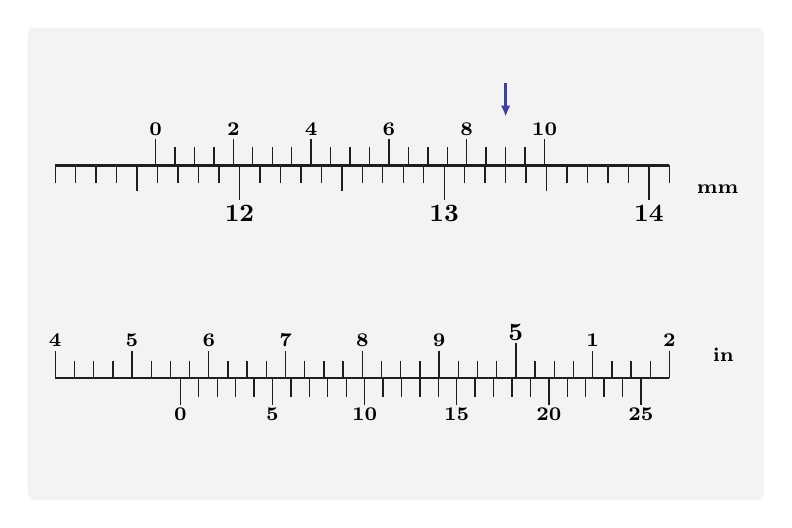
\begin{tikzpicture}[scale=1]
  \fill[figpanel,rounded corners=2pt] (-0.35,-1.55) rectangle (9,4.45);
  \begin{scope}[yshift=2.70cm]
  \draw[scb] (0,0) -- (7.8,0);
  \draw[sc] (0,0) -- (0,-0.22);
  \draw[sc] (0.26,0) -- (0.26,-0.22);
  \draw[sc] (0.52,0) -- (0.52,-0.22);
  \draw[sc] (0.78,0) -- (0.78,-0.22);
  \draw[sc] (1.04,0) -- (1.04,-0.32);
  \draw[sc] (1.3,0) -- (1.3,-0.22);
  \draw[sc] (1.56,0) -- (1.56,-0.22);
  \draw[sc] (1.82,0) -- (1.82,-0.22);
  \draw[sc] (2.08,0) -- (2.08,-0.22);
  \draw[sc] (2.34,0) -- (2.34,-0.44);
  \node[lab,below] at (2.34,-0.46) {12};
  \draw[sc] (2.6,0) -- (2.6,-0.22);
  \draw[sc] (2.86,0) -- (2.86,-0.22);
  \draw[sc] (3.12,0) -- (3.12,-0.22);
  \draw[sc] (3.38,0) -- (3.38,-0.22);
  \draw[sc] (3.64,0) -- (3.64,-0.32);
  \draw[sc] (3.9,0) -- (3.9,-0.22);
  \draw[sc] (4.16,0) -- (4.16,-0.22);
  \draw[sc] (4.42,0) -- (4.42,-0.22);
  \draw[sc] (4.68,0) -- (4.68,-0.22);
  \draw[sc] (4.94,0) -- (4.94,-0.44);
  \node[lab,below] at (4.94,-0.46) {13};
  \draw[sc] (5.2,0) -- (5.2,-0.22);
  \draw[sc] (5.46,0) -- (5.46,-0.22);
  \draw[sc] (5.72,0) -- (5.72,-0.22);
  \draw[sc] (5.98,0) -- (5.98,-0.22);
  \draw[sc] (6.24,0) -- (6.24,-0.32);
  \draw[sc] (6.5,0) -- (6.5,-0.22);
  \draw[sc] (6.76,0) -- (6.76,-0.22);
  \draw[sc] (7.02,0) -- (7.02,-0.22);
  \draw[sc] (7.28,0) -- (7.28,-0.22);
  \draw[sc] (7.54,0) -- (7.54,-0.44);
  \node[lab,below] at (7.54,-0.46) {14};
  \draw[sc] (7.8,0) -- (7.8,-0.22);
  \draw[sc] (1.274,0) -- (1.274,0.34);
  \node[labs,above] at (1.274,0.34) {0};
  \draw[sc] (1.521,0) -- (1.521,0.24);
  \draw[sc] (1.768,0) -- (1.768,0.24);
  \draw[sc] (2.015,0) -- (2.015,0.24);
  \draw[sc] (2.262,0) -- (2.262,0.34);
  \node[labs,above] at (2.262,0.34) {2};
  \draw[sc] (2.509,0) -- (2.509,0.24);
  \draw[sc] (2.756,0) -- (2.756,0.24);
  \draw[sc] (3.003,0) -- (3.003,0.24);
  \draw[sc] (3.25,0) -- (3.25,0.34);
  \node[labs,above] at (3.25,0.34) {4};
  \draw[sc] (3.497,0) -- (3.497,0.24);
  \draw[sc] (3.744,0) -- (3.744,0.24);
  \draw[sc] (3.991,0) -- (3.991,0.24);
  \draw[sc] (4.238,0) -- (4.238,0.34);
  \node[labs,above] at (4.238,0.34) {6};
  \draw[sc] (4.485,0) -- (4.485,0.24);
  \draw[sc] (4.732,0) -- (4.732,0.24);
  \draw[sc] (4.979,0) -- (4.979,0.24);
  \draw[sc] (5.226,0) -- (5.226,0.34);
  \node[labs,above] at (5.226,0.34) {8};
  \draw[sc] (5.473,0) -- (5.473,0.24);
  \draw[sc] (5.72,0) -- (5.72,0.24);
  \draw[sc] (5.967,0) -- (5.967,0.24);
  \draw[sc] (6.214,0) -- (6.214,0.34);
  \node[labs,above] at (6.214,0.34) {10};
  \draw[ptr] (5.72,1.05) -- (5.72,0.62);
  \node[labs,left] at (8.72,-0.30) {mm};
  \end{scope}
  \begin{scope}[yshift=0cm]
  \draw[scb] (0,0) -- (7.8,0);
  \draw[sc] (0,0) -- (0,0.34);
  \node[labs,above] at (0,0.36) {4};
  \draw[sc] (0.2437,0) -- (0.2437,0.22);
  \draw[sc] (0.4875,0) -- (0.4875,0.22);
  \draw[sc] (0.7313,0) -- (0.7313,0.22);
  \draw[sc] (0.975,0) -- (0.975,0.34);
  \node[labs,above] at (0.975,0.36) {5};
  \draw[sc] (1.2188,0) -- (1.2188,0.22);
  \draw[sc] (1.4625,0) -- (1.4625,0.22);
  \draw[sc] (1.7062,0) -- (1.7062,0.22);
  \draw[sc] (1.95,0) -- (1.95,0.34);
  \node[labs,above] at (1.95,0.36) {6};
  \draw[sc] (2.1937,0) -- (2.1937,0.22);
  \draw[sc] (2.4375,0) -- (2.4375,0.22);
  \draw[sc] (2.6812,0) -- (2.6812,0.22);
  \draw[sc] (2.925,0) -- (2.925,0.34);
  \node[labs,above] at (2.925,0.36) {7};
  \draw[sc] (3.1688,0) -- (3.1688,0.22);
  \draw[sc] (3.4125,0) -- (3.4125,0.22);
  \draw[sc] (3.6562,0) -- (3.6562,0.22);
  \draw[sc] (3.9,0) -- (3.9,0.34);
  \node[labs,above] at (3.9,0.36) {8};
  \draw[sc] (4.1437,0) -- (4.1437,0.22);
  \draw[sc] (4.3875,0) -- (4.3875,0.22);
  \draw[sc] (4.6312,0) -- (4.6312,0.22);
  \draw[sc] (4.875,0) -- (4.875,0.34);
  \node[labs,above] at (4.875,0.36) {9};
  \draw[sc] (5.1188,0) -- (5.1188,0.22);
  \draw[sc] (5.3625,0) -- (5.3625,0.22);
  \draw[sc] (5.6063,0) -- (5.6063,0.22);
  \draw[sc] (5.85,0) -- (5.85,0.44);
  \node[lab,above] at (5.85,0.44) {5};
  \draw[sc] (6.0938,0) -- (6.0938,0.22);
  \draw[sc] (6.3375,0) -- (6.3375,0.22);
  \draw[sc] (6.5812,0) -- (6.5812,0.22);
  \draw[sc] (6.825,0) -- (6.825,0.34);
  \node[labs,above] at (6.825,0.36) {1};
  \draw[sc] (7.0687,0) -- (7.0687,0.22);
  \draw[sc] (7.3125,0) -- (7.3125,0.22);
  \draw[sc] (7.5563,0) -- (7.5563,0.22);
  \draw[sc] (7.8,0) -- (7.8,0.34);
  \node[labs,above] at (7.8,0.36) {2};
  \draw[sc] (1.5892,0) -- (1.5892,-0.34);
  \node[labs,below] at (1.5892,-0.34) {0};
  \draw[sc] (1.8232,0) -- (1.8232,-0.24);
  \draw[sc] (2.0572,0) -- (2.0572,-0.24);
  \draw[sc] (2.2912,0) -- (2.2912,-0.24);
  \draw[sc] (2.5252,0) -- (2.5252,-0.24);
  \draw[sc] (2.7592,0) -- (2.7592,-0.34);
  \node[labs,below] at (2.7592,-0.34) {5};
  \draw[sc] (2.9932,0) -- (2.9932,-0.24);
  \draw[sc] (3.2272,0) -- (3.2272,-0.24);
  \draw[sc] (3.4612,0) -- (3.4612,-0.24);
  \draw[sc] (3.6952,0) -- (3.6952,-0.24);
  \draw[sc] (3.9292,0) -- (3.9292,-0.34);
  \node[labs,below] at (3.9292,-0.34) {10};
  \draw[sc] (4.1632,0) -- (4.1632,-0.24);
  \draw[sc] (4.3972,0) -- (4.3972,-0.24);
  \draw[sc] (4.6312,0) -- (4.6312,-0.24);
  \draw[sc] (4.8652,0) -- (4.8652,-0.24);
  \draw[sc] (5.0992,0) -- (5.0992,-0.34);
  \node[labs,below] at (5.0992,-0.34) {15};
  \draw[sc] (5.3332,0) -- (5.3332,-0.24);
  \draw[sc] (5.5672,0) -- (5.5672,-0.24);
  \draw[sc] (5.8012,0) -- (5.8012,-0.24);
  \draw[sc] (6.0352,0) -- (6.0352,-0.24);
  \draw[sc] (6.2692,0) -- (6.2692,-0.34);
  \node[labs,below] at (6.2692,-0.34) {20};
  \draw[sc] (6.5032,0) -- (6.5032,-0.24);
  \draw[sc] (6.7372,0) -- (6.7372,-0.24);
  \draw[sc] (6.9712,0) -- (6.9712,-0.24);
  \draw[sc] (7.2052,0) -- (7.2052,-0.24);
  \draw[sc] (7.4392,0) -- (7.4392,-0.34);
  \node[labs,below] at (7.4392,-0.34) {25};
  \node[labs,left] at (8.66,0.30) {in};
  \end{scope}
\end{tikzpicture}
}

\newcommand{\figQBB}{%
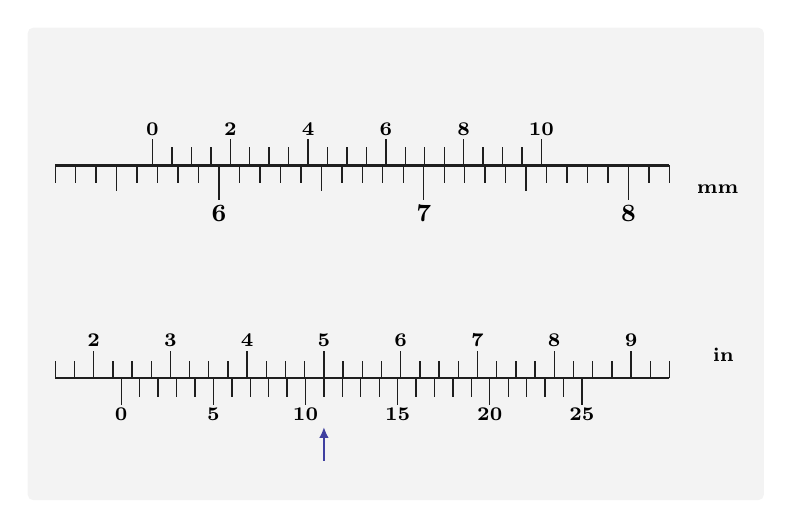
\begin{tikzpicture}[scale=1]
  \fill[figpanel,rounded corners=2pt] (-0.35,-1.55) rectangle (9,4.45);
  \begin{scope}[yshift=2.70cm]
  \draw[scb] (0,0) -- (7.8,0);
  \draw[sc] (0,0) -- (0,-0.22);
  \draw[sc] (0.26,0) -- (0.26,-0.22);
  \draw[sc] (0.52,0) -- (0.52,-0.22);
  \draw[sc] (0.78,0) -- (0.78,-0.32);
  \draw[sc] (1.04,0) -- (1.04,-0.22);
  \draw[sc] (1.3,0) -- (1.3,-0.22);
  \draw[sc] (1.56,0) -- (1.56,-0.22);
  \draw[sc] (1.82,0) -- (1.82,-0.22);
  \draw[sc] (2.08,0) -- (2.08,-0.44);
  \node[lab,below] at (2.08,-0.46) {6};
  \draw[sc] (2.34,0) -- (2.34,-0.22);
  \draw[sc] (2.6,0) -- (2.6,-0.22);
  \draw[sc] (2.86,0) -- (2.86,-0.22);
  \draw[sc] (3.12,0) -- (3.12,-0.22);
  \draw[sc] (3.38,0) -- (3.38,-0.32);
  \draw[sc] (3.64,0) -- (3.64,-0.22);
  \draw[sc] (3.9,0) -- (3.9,-0.22);
  \draw[sc] (4.16,0) -- (4.16,-0.22);
  \draw[sc] (4.42,0) -- (4.42,-0.22);
  \draw[sc] (4.68,0) -- (4.68,-0.44);
  \node[lab,below] at (4.68,-0.46) {7};
  \draw[sc] (4.94,0) -- (4.94,-0.22);
  \draw[sc] (5.2,0) -- (5.2,-0.22);
  \draw[sc] (5.46,0) -- (5.46,-0.22);
  \draw[sc] (5.72,0) -- (5.72,-0.22);
  \draw[sc] (5.98,0) -- (5.98,-0.32);
  \draw[sc] (6.24,0) -- (6.24,-0.22);
  \draw[sc] (6.5,0) -- (6.5,-0.22);
  \draw[sc] (6.76,0) -- (6.76,-0.22);
  \draw[sc] (7.02,0) -- (7.02,-0.22);
  \draw[sc] (7.28,0) -- (7.28,-0.44);
  \node[lab,below] at (7.28,-0.46) {8};
  \draw[sc] (7.54,0) -- (7.54,-0.22);
  \draw[sc] (7.8,0) -- (7.8,-0.22);
  \draw[sc] (1.235,0) -- (1.235,0.34);
  \node[labs,above] at (1.235,0.34) {0};
  \draw[sc] (1.482,0) -- (1.482,0.24);
  \draw[sc] (1.729,0) -- (1.729,0.24);
  \draw[sc] (1.976,0) -- (1.976,0.24);
  \draw[sc] (2.223,0) -- (2.223,0.34);
  \node[labs,above] at (2.223,0.34) {2};
  \draw[sc] (2.47,0) -- (2.47,0.24);
  \draw[sc] (2.717,0) -- (2.717,0.24);
  \draw[sc] (2.964,0) -- (2.964,0.24);
  \draw[sc] (3.211,0) -- (3.211,0.34);
  \node[labs,above] at (3.211,0.34) {4};
  \draw[sc] (3.458,0) -- (3.458,0.24);
  \draw[sc] (3.705,0) -- (3.705,0.24);
  \draw[sc] (3.952,0) -- (3.952,0.24);
  \draw[sc] (4.199,0) -- (4.199,0.34);
  \node[labs,above] at (4.199,0.34) {6};
  \draw[sc] (4.446,0) -- (4.446,0.24);
  \draw[sc] (4.693,0) -- (4.693,0.24);
  \draw[sc] (4.94,0) -- (4.94,0.24);
  \draw[sc] (5.187,0) -- (5.187,0.34);
  \node[labs,above] at (5.187,0.34) {8};
  \draw[sc] (5.434,0) -- (5.434,0.24);
  \draw[sc] (5.681,0) -- (5.681,0.24);
  \draw[sc] (5.928,0) -- (5.928,0.24);
  \draw[sc] (6.175,0) -- (6.175,0.34);
  \node[labs,above] at (6.175,0.34) {10};
  \node[labs,left] at (8.72,-0.30) {mm};
  \end{scope}
  \begin{scope}[yshift=0cm]
  \draw[scb] (0,0) -- (7.8,0);
  \draw[sc] (0,0) -- (0,0.22);
  \draw[sc] (0.2438,0) -- (0.2438,0.22);
  \draw[sc] (0.4875,0) -- (0.4875,0.34);
  \node[labs,above] at (0.4875,0.36) {2};
  \draw[sc] (0.7313,0) -- (0.7313,0.22);
  \draw[sc] (0.975,0) -- (0.975,0.22);
  \draw[sc] (1.2188,0) -- (1.2188,0.22);
  \draw[sc] (1.4625,0) -- (1.4625,0.34);
  \node[labs,above] at (1.4625,0.36) {3};
  \draw[sc] (1.7063,0) -- (1.7063,0.22);
  \draw[sc] (1.95,0) -- (1.95,0.22);
  \draw[sc] (2.1938,0) -- (2.1938,0.22);
  \draw[sc] (2.4375,0) -- (2.4375,0.34);
  \node[labs,above] at (2.4375,0.36) {4};
  \draw[sc] (2.6813,0) -- (2.6813,0.22);
  \draw[sc] (2.925,0) -- (2.925,0.22);
  \draw[sc] (3.1688,0) -- (3.1688,0.22);
  \draw[sc] (3.4125,0) -- (3.4125,0.34);
  \node[labs,above] at (3.4125,0.36) {5};
  \draw[sc] (3.6563,0) -- (3.6563,0.22);
  \draw[sc] (3.9,0) -- (3.9,0.22);
  \draw[sc] (4.1438,0) -- (4.1438,0.22);
  \draw[sc] (4.3875,0) -- (4.3875,0.34);
  \node[labs,above] at (4.3875,0.36) {6};
  \draw[sc] (4.6313,0) -- (4.6313,0.22);
  \draw[sc] (4.875,0) -- (4.875,0.22);
  \draw[sc] (5.1188,0) -- (5.1188,0.22);
  \draw[sc] (5.3625,0) -- (5.3625,0.34);
  \node[labs,above] at (5.3625,0.36) {7};
  \draw[sc] (5.6063,0) -- (5.6063,0.22);
  \draw[sc] (5.85,0) -- (5.85,0.22);
  \draw[sc] (6.0938,0) -- (6.0938,0.22);
  \draw[sc] (6.3375,0) -- (6.3375,0.34);
  \node[labs,above] at (6.3375,0.36) {8};
  \draw[sc] (6.5813,0) -- (6.5813,0.22);
  \draw[sc] (6.825,0) -- (6.825,0.22);
  \draw[sc] (7.0688,0) -- (7.0688,0.22);
  \draw[sc] (7.3125,0) -- (7.3125,0.34);
  \node[labs,above] at (7.3125,0.36) {9};
  \draw[sc] (7.5563,0) -- (7.5563,0.22);
  \draw[sc] (7.8,0) -- (7.8,0.22);
  \draw[sc] (0.8385,0) -- (0.8385,-0.34);
  \node[labs,below] at (0.8385,-0.34) {0};
  \draw[sc] (1.0725,0) -- (1.0725,-0.24);
  \draw[sc] (1.3065,0) -- (1.3065,-0.24);
  \draw[sc] (1.5405,0) -- (1.5405,-0.24);
  \draw[sc] (1.7745,0) -- (1.7745,-0.24);
  \draw[sc] (2.0085,0) -- (2.0085,-0.34);
  \node[labs,below] at (2.0085,-0.34) {5};
  \draw[sc] (2.2425,0) -- (2.2425,-0.24);
  \draw[sc] (2.4765,0) -- (2.4765,-0.24);
  \draw[sc] (2.7105,0) -- (2.7105,-0.24);
  \draw[sc] (2.9445,0) -- (2.9445,-0.24);
  \draw[sc] (3.1785,0) -- (3.1785,-0.34);
  \node[labs,below] at (3.1785,-0.34) {10};
  \draw[sc] (3.4125,0) -- (3.4125,-0.24);
  \draw[sc] (3.6465,0) -- (3.6465,-0.24);
  \draw[sc] (3.8805,0) -- (3.8805,-0.24);
  \draw[sc] (4.1145,0) -- (4.1145,-0.24);
  \draw[sc] (4.3485,0) -- (4.3485,-0.34);
  \node[labs,below] at (4.3485,-0.34) {15};
  \draw[sc] (4.5825,0) -- (4.5825,-0.24);
  \draw[sc] (4.8165,0) -- (4.8165,-0.24);
  \draw[sc] (5.0505,0) -- (5.0505,-0.24);
  \draw[sc] (5.2845,0) -- (5.2845,-0.24);
  \draw[sc] (5.5185,0) -- (5.5185,-0.34);
  \node[labs,below] at (5.5185,-0.34) {20};
  \draw[sc] (5.7525,0) -- (5.7525,-0.24);
  \draw[sc] (5.9865,0) -- (5.9865,-0.24);
  \draw[sc] (6.2205,0) -- (6.2205,-0.24);
  \draw[sc] (6.4545,0) -- (6.4545,-0.24);
  \draw[sc] (6.6885,0) -- (6.6885,-0.34);
  \node[labs,below] at (6.6885,-0.34) {25};
  \draw[ptr] (3.4125,-1.05) -- (3.4125,-0.62);
  \node[labs,left] at (8.66,0.30) {in};
  \end{scope}
\end{tikzpicture}
}

\newcommand{\figQBC}{%
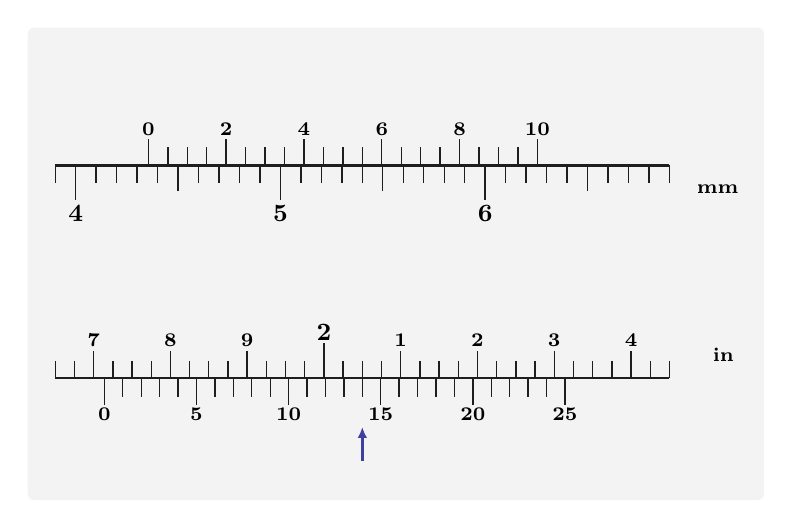
\begin{tikzpicture}[scale=1]
  \fill[figpanel,rounded corners=2pt] (-0.35,-1.55) rectangle (9,4.45);
  \begin{scope}[yshift=2.70cm]
  \draw[scb] (0,0) -- (7.8,0);
  \draw[sc] (0,0) -- (0,-0.22);
  \draw[sc] (0.26,0) -- (0.26,-0.44);
  \node[lab,below] at (0.26,-0.46) {4};
  \draw[sc] (0.52,0) -- (0.52,-0.22);
  \draw[sc] (0.78,0) -- (0.78,-0.22);
  \draw[sc] (1.04,0) -- (1.04,-0.22);
  \draw[sc] (1.3,0) -- (1.3,-0.22);
  \draw[sc] (1.56,0) -- (1.56,-0.32);
  \draw[sc] (1.82,0) -- (1.82,-0.22);
  \draw[sc] (2.08,0) -- (2.08,-0.22);
  \draw[sc] (2.34,0) -- (2.34,-0.22);
  \draw[sc] (2.6,0) -- (2.6,-0.22);
  \draw[sc] (2.86,0) -- (2.86,-0.44);
  \node[lab,below] at (2.86,-0.46) {5};
  \draw[sc] (3.12,0) -- (3.12,-0.22);
  \draw[sc] (3.38,0) -- (3.38,-0.22);
  \draw[sc] (3.64,0) -- (3.64,-0.22);
  \draw[sc] (3.9,0) -- (3.9,-0.22);
  \draw[sc] (4.16,0) -- (4.16,-0.32);
  \draw[sc] (4.42,0) -- (4.42,-0.22);
  \draw[sc] (4.68,0) -- (4.68,-0.22);
  \draw[sc] (4.94,0) -- (4.94,-0.22);
  \draw[sc] (5.2,0) -- (5.2,-0.22);
  \draw[sc] (5.46,0) -- (5.46,-0.44);
  \node[lab,below] at (5.46,-0.46) {6};
  \draw[sc] (5.72,0) -- (5.72,-0.22);
  \draw[sc] (5.98,0) -- (5.98,-0.22);
  \draw[sc] (6.24,0) -- (6.24,-0.22);
  \draw[sc] (6.5,0) -- (6.5,-0.22);
  \draw[sc] (6.76,0) -- (6.76,-0.32);
  \draw[sc] (7.02,0) -- (7.02,-0.22);
  \draw[sc] (7.28,0) -- (7.28,-0.22);
  \draw[sc] (7.54,0) -- (7.54,-0.22);
  \draw[sc] (7.8,0) -- (7.8,-0.22);
  \draw[sc] (1.183,0) -- (1.183,0.34);
  \node[labs,above] at (1.183,0.34) {0};
  \draw[sc] (1.43,0) -- (1.43,0.24);
  \draw[sc] (1.677,0) -- (1.677,0.24);
  \draw[sc] (1.924,0) -- (1.924,0.24);
  \draw[sc] (2.171,0) -- (2.171,0.34);
  \node[labs,above] at (2.171,0.34) {2};
  \draw[sc] (2.418,0) -- (2.418,0.24);
  \draw[sc] (2.665,0) -- (2.665,0.24);
  \draw[sc] (2.912,0) -- (2.912,0.24);
  \draw[sc] (3.159,0) -- (3.159,0.34);
  \node[labs,above] at (3.159,0.34) {4};
  \draw[sc] (3.406,0) -- (3.406,0.24);
  \draw[sc] (3.653,0) -- (3.653,0.24);
  \draw[sc] (3.9,0) -- (3.9,0.24);
  \draw[sc] (4.147,0) -- (4.147,0.34);
  \node[labs,above] at (4.147,0.34) {6};
  \draw[sc] (4.394,0) -- (4.394,0.24);
  \draw[sc] (4.641,0) -- (4.641,0.24);
  \draw[sc] (4.888,0) -- (4.888,0.24);
  \draw[sc] (5.135,0) -- (5.135,0.34);
  \node[labs,above] at (5.135,0.34) {8};
  \draw[sc] (5.382,0) -- (5.382,0.24);
  \draw[sc] (5.629,0) -- (5.629,0.24);
  \draw[sc] (5.876,0) -- (5.876,0.24);
  \draw[sc] (6.123,0) -- (6.123,0.34);
  \node[labs,above] at (6.123,0.34) {10};
  \node[labs,left] at (8.72,-0.30) {mm};
  \end{scope}
  \begin{scope}[yshift=0cm]
  \draw[scb] (0,0) -- (7.8,0);
  \draw[sc] (0,0) -- (0,0.22);
  \draw[sc] (0.2438,0) -- (0.2438,0.22);
  \draw[sc] (0.4875,0) -- (0.4875,0.34);
  \node[labs,above] at (0.4875,0.36) {7};
  \draw[sc] (0.7313,0) -- (0.7313,0.22);
  \draw[sc] (0.975,0) -- (0.975,0.22);
  \draw[sc] (1.2188,0) -- (1.2188,0.22);
  \draw[sc] (1.4625,0) -- (1.4625,0.34);
  \node[labs,above] at (1.4625,0.36) {8};
  \draw[sc] (1.7063,0) -- (1.7063,0.22);
  \draw[sc] (1.95,0) -- (1.95,0.22);
  \draw[sc] (2.1938,0) -- (2.1938,0.22);
  \draw[sc] (2.4375,0) -- (2.4375,0.34);
  \node[labs,above] at (2.4375,0.36) {9};
  \draw[sc] (2.6813,0) -- (2.6813,0.22);
  \draw[sc] (2.925,0) -- (2.925,0.22);
  \draw[sc] (3.1688,0) -- (3.1688,0.22);
  \draw[sc] (3.4125,0) -- (3.4125,0.44);
  \node[lab,above] at (3.4125,0.44) {2};
  \draw[sc] (3.6562,0) -- (3.6562,0.22);
  \draw[sc] (3.9,0) -- (3.9,0.22);
  \draw[sc] (4.1438,0) -- (4.1438,0.22);
  \draw[sc] (4.3875,0) -- (4.3875,0.34);
  \node[labs,above] at (4.3875,0.36) {1};
  \draw[sc] (4.6313,0) -- (4.6313,0.22);
  \draw[sc] (4.875,0) -- (4.875,0.22);
  \draw[sc] (5.1188,0) -- (5.1188,0.22);
  \draw[sc] (5.3625,0) -- (5.3625,0.34);
  \node[labs,above] at (5.3625,0.36) {2};
  \draw[sc] (5.6063,0) -- (5.6063,0.22);
  \draw[sc] (5.85,0) -- (5.85,0.22);
  \draw[sc] (6.0938,0) -- (6.0938,0.22);
  \draw[sc] (6.3375,0) -- (6.3375,0.34);
  \node[labs,above] at (6.3375,0.36) {3};
  \draw[sc] (6.5813,0) -- (6.5813,0.22);
  \draw[sc] (6.825,0) -- (6.825,0.22);
  \draw[sc] (7.0688,0) -- (7.0688,0.22);
  \draw[sc] (7.3125,0) -- (7.3125,0.34);
  \node[labs,above] at (7.3125,0.36) {4};
  \draw[sc] (7.5563,0) -- (7.5563,0.22);
  \draw[sc] (7.8,0) -- (7.8,0.22);
  \draw[sc] (0.624,0) -- (0.624,-0.34);
  \node[labs,below] at (0.624,-0.34) {0};
  \draw[sc] (0.858,0) -- (0.858,-0.24);
  \draw[sc] (1.092,0) -- (1.092,-0.24);
  \draw[sc] (1.326,0) -- (1.326,-0.24);
  \draw[sc] (1.56,0) -- (1.56,-0.24);
  \draw[sc] (1.794,0) -- (1.794,-0.34);
  \node[labs,below] at (1.794,-0.34) {5};
  \draw[sc] (2.028,0) -- (2.028,-0.24);
  \draw[sc] (2.262,0) -- (2.262,-0.24);
  \draw[sc] (2.496,0) -- (2.496,-0.24);
  \draw[sc] (2.73,0) -- (2.73,-0.24);
  \draw[sc] (2.964,0) -- (2.964,-0.34);
  \node[labs,below] at (2.964,-0.34) {10};
  \draw[sc] (3.198,0) -- (3.198,-0.24);
  \draw[sc] (3.432,0) -- (3.432,-0.24);
  \draw[sc] (3.666,0) -- (3.666,-0.24);
  \draw[sc] (3.9,0) -- (3.9,-0.24);
  \draw[sc] (4.134,0) -- (4.134,-0.34);
  \node[labs,below] at (4.134,-0.34) {15};
  \draw[sc] (4.368,0) -- (4.368,-0.24);
  \draw[sc] (4.602,0) -- (4.602,-0.24);
  \draw[sc] (4.836,0) -- (4.836,-0.24);
  \draw[sc] (5.07,0) -- (5.07,-0.24);
  \draw[sc] (5.304,0) -- (5.304,-0.34);
  \node[labs,below] at (5.304,-0.34) {20};
  \draw[sc] (5.538,0) -- (5.538,-0.24);
  \draw[sc] (5.772,0) -- (5.772,-0.24);
  \draw[sc] (6.006,0) -- (6.006,-0.24);
  \draw[sc] (6.24,0) -- (6.24,-0.24);
  \draw[sc] (6.474,0) -- (6.474,-0.34);
  \node[labs,below] at (6.474,-0.34) {25};
  \draw[ptr] (3.9,-1.05) -- (3.9,-0.62);
  \node[labs,left] at (8.66,0.30) {in};
  \end{scope}
\end{tikzpicture}
}

\newcommand{\figQBF}{%
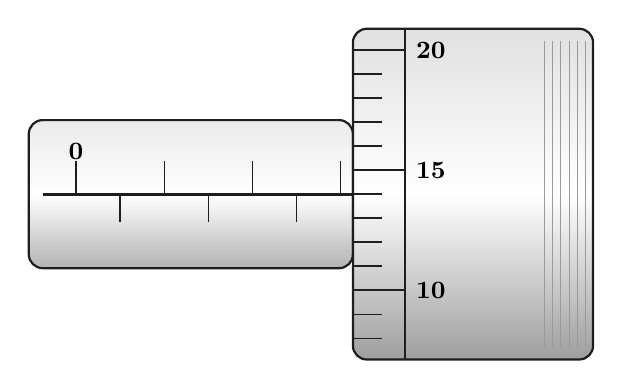
\begin{tikzpicture}[scale=1]
  \shade[rounded corners=5pt,top color=black!8,bottom color=black!30,middle color=white] (0,-0.94) rectangle (4.1168,0.94);
  \draw[scb,rounded corners=5pt] (0,-0.94) rectangle (4.1168,0.94);
  \draw[draw=figline,line width=1.1pt] (0.18,0) -- (4.1168,0);
  \draw[sc] (0.6,0) -- (0.6,0.42);
  \node[lab,above] at (0.6,0.40) {0};
  \draw[sc] (1.16,0) -- (1.16,-0.36);
  \draw[sc] (1.72,0) -- (1.72,0.42);
  \draw[sc] (2.28,0) -- (2.28,-0.36);
  \draw[sc] (2.84,0) -- (2.84,0.42);
  \draw[sc] (3.4,0) -- (3.4,-0.36);
  \draw[sc] (3.96,0) -- (3.96,0.42);
  \shade[rounded corners=5pt,top color=black!12,bottom color=black!38,middle color=white] (4.1168,-2.1) rectangle (7.1668,2.1);
  \draw[scb,rounded corners=5pt] (4.1168,-2.1) rectangle (7.1668,2.1);
  \draw[draw=figline,line width=1.0pt] (4.1168,-1.94) -- (4.1168,1.94);
  \draw[sc] (4.7768,-2.1) -- (4.7768,2.1);
  \draw[draw=figline!45,line width=0.4pt] (6.5468,-1.94) -- (6.5468,1.94);
  \draw[draw=figline!45,line width=0.4pt] (6.6518,-1.94) -- (6.6518,1.94);
  \draw[draw=figline!45,line width=0.4pt] (6.7568,-1.94) -- (6.7568,1.94);
  \draw[draw=figline!45,line width=0.4pt] (6.8618,-1.94) -- (6.8618,1.94);
  \draw[draw=figline!45,line width=0.4pt] (6.9668,-1.94) -- (6.9668,1.94);
  \draw[draw=figline!45,line width=0.4pt] (7.0718,-1.94) -- (7.0718,1.94);
  \draw[draw=figline,line width=0.5pt] (4.1168,-1.83) -- (4.4798,-1.83);
  \draw[draw=figline,line width=0.5pt] (4.1168,-1.525) -- (4.4798,-1.525);
  \draw[draw=figline,line width=0.9pt] (4.1168,-1.22) -- (4.7768,-1.22);
  \node[lab,right] at (4.8768,-1.22) {10};
  \draw[draw=figline,line width=0.5pt] (4.1168,-0.915) -- (4.4798,-0.915);
  \draw[draw=figline,line width=0.5pt] (4.1168,-0.61) -- (4.4798,-0.61);
  \draw[draw=figline,line width=0.5pt] (4.1168,-0.305) -- (4.4798,-0.305);
  \draw[draw=figline,line width=0.5pt] (4.1168,0) -- (4.4798,0);
  \draw[draw=figline,line width=0.9pt] (4.1168,0.305) -- (4.7768,0.305);
  \node[lab,right] at (4.8768,0.305) {15};
  \draw[draw=figline,line width=0.5pt] (4.1168,0.61) -- (4.4798,0.61);
  \draw[draw=figline,line width=0.5pt] (4.1168,0.915) -- (4.4798,0.915);
  \draw[draw=figline,line width=0.5pt] (4.1168,1.22) -- (4.4798,1.22);
  \draw[draw=figline,line width=0.5pt] (4.1168,1.525) -- (4.4798,1.525);
  \draw[draw=figline,line width=0.9pt] (4.1168,1.83) -- (4.7768,1.83);
  \node[lab,right] at (4.8768,1.83) {20};
\end{tikzpicture}
}

\newcommand{\figQBG}{%
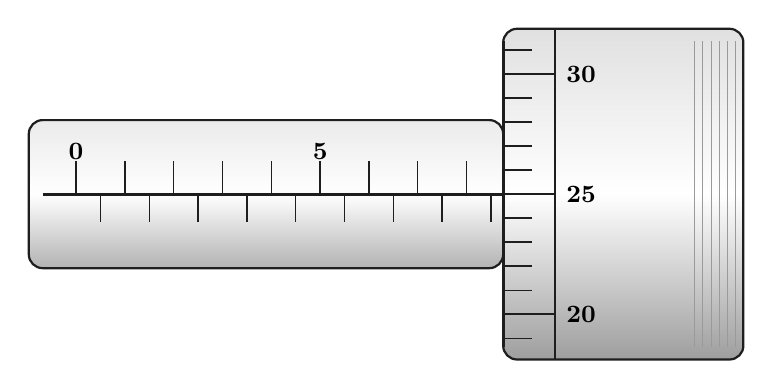
\begin{tikzpicture}[scale=1]
  \shade[rounded corners=5pt,top color=black!8,bottom color=black!30,middle color=white] (0,-0.94) rectangle (6.025,0.94);
  \draw[scb,rounded corners=5pt] (0,-0.94) rectangle (6.025,0.94);
  \draw[draw=figline,line width=1.1pt] (0.18,0) -- (6.025,0);
  \draw[sc] (0.6,0) -- (0.6,0.42);
  \node[lab,above] at (0.6,0.40) {0};
  \draw[sc] (0.91,0) -- (0.91,-0.36);
  \draw[sc] (1.22,0) -- (1.22,0.42);
  \draw[sc] (1.53,0) -- (1.53,-0.36);
  \draw[sc] (1.84,0) -- (1.84,0.42);
  \draw[sc] (2.15,0) -- (2.15,-0.36);
  \draw[sc] (2.46,0) -- (2.46,0.42);
  \draw[sc] (2.77,0) -- (2.77,-0.36);
  \draw[sc] (3.08,0) -- (3.08,0.42);
  \draw[sc] (3.39,0) -- (3.39,-0.36);
  \draw[sc] (3.7,0) -- (3.7,0.42);
  \node[lab,above] at (3.7,0.40) {5};
  \draw[sc] (4.01,0) -- (4.01,-0.36);
  \draw[sc] (4.32,0) -- (4.32,0.42);
  \draw[sc] (4.63,0) -- (4.63,-0.36);
  \draw[sc] (4.94,0) -- (4.94,0.42);
  \draw[sc] (5.25,0) -- (5.25,-0.36);
  \draw[sc] (5.56,0) -- (5.56,0.42);
  \draw[sc] (5.87,0) -- (5.87,-0.36);
  \shade[rounded corners=5pt,top color=black!12,bottom color=black!38,middle color=white] (6.025,-2.1) rectangle (9.075,2.1);
  \draw[scb,rounded corners=5pt] (6.025,-2.1) rectangle (9.075,2.1);
  \draw[draw=figline,line width=1.0pt] (6.025,-1.94) -- (6.025,1.94);
  \draw[sc] (6.685,-2.1) -- (6.685,2.1);
  \draw[draw=figline!45,line width=0.4pt] (8.455,-1.94) -- (8.455,1.94);
  \draw[draw=figline!45,line width=0.4pt] (8.56,-1.94) -- (8.56,1.94);
  \draw[draw=figline!45,line width=0.4pt] (8.665,-1.94) -- (8.665,1.94);
  \draw[draw=figline!45,line width=0.4pt] (8.77,-1.94) -- (8.77,1.94);
  \draw[draw=figline!45,line width=0.4pt] (8.875,-1.94) -- (8.875,1.94);
  \draw[draw=figline!45,line width=0.4pt] (8.98,-1.94) -- (8.98,1.94);
  \draw[draw=figline,line width=0.5pt] (6.025,-1.83) -- (6.388,-1.83);
  \draw[draw=figline,line width=0.9pt] (6.025,-1.525) -- (6.685,-1.525);
  \node[lab,right] at (6.785,-1.525) {20};
  \draw[draw=figline,line width=0.5pt] (6.025,-1.22) -- (6.388,-1.22);
  \draw[draw=figline,line width=0.5pt] (6.025,-0.915) -- (6.388,-0.915);
  \draw[draw=figline,line width=0.5pt] (6.025,-0.61) -- (6.388,-0.61);
  \draw[draw=figline,line width=0.5pt] (6.025,-0.305) -- (6.388,-0.305);
  \draw[draw=figline,line width=0.9pt] (6.025,0) -- (6.685,0);
  \node[lab,right] at (6.785,0) {25};
  \draw[draw=figline,line width=0.5pt] (6.025,0.305) -- (6.388,0.305);
  \draw[draw=figline,line width=0.5pt] (6.025,0.61) -- (6.388,0.61);
  \draw[draw=figline,line width=0.5pt] (6.025,0.915) -- (6.388,0.915);
  \draw[draw=figline,line width=0.5pt] (6.025,1.22) -- (6.388,1.22);
  \draw[draw=figline,line width=0.9pt] (6.025,1.525) -- (6.685,1.525);
  \node[lab,right] at (6.785,1.525) {30};
  \draw[draw=figline,line width=0.5pt] (6.025,1.83) -- (6.388,1.83);
\end{tikzpicture}
}

\newcommand{\figQBH}{%
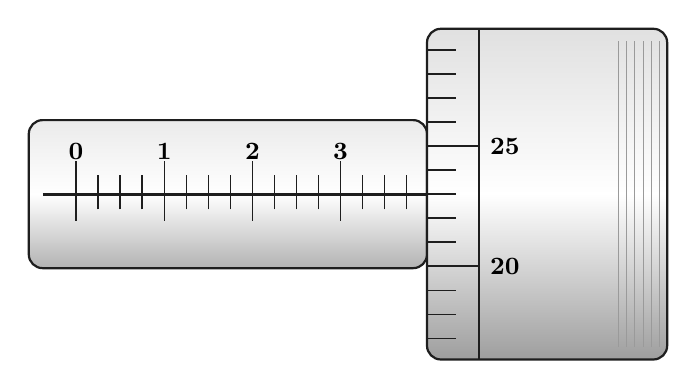
\begin{tikzpicture}[scale=1]
  \shade[rounded corners=5pt,top color=black!8,bottom color=black!30,middle color=white] (0,-0.94) rectangle (5.0576,0.94);
  \draw[scb,rounded corners=5pt] (0,-0.94) rectangle (5.0576,0.94);
  \draw[draw=figline,line width=1.1pt] (0.18,0) -- (5.0576,0);
  \draw[sc] (0.6,-0.336) -- (0.6,0.42);
  \node[lab,above] at (0.6,0.40) {0};
  \draw[sc] (0.88,-0.192) -- (0.88,0.24);
  \draw[sc] (1.16,-0.192) -- (1.16,0.24);
  \draw[sc] (1.44,-0.192) -- (1.44,0.24);
  \draw[sc] (1.72,-0.336) -- (1.72,0.42);
  \node[lab,above] at (1.72,0.40) {1};
  \draw[sc] (2,-0.192) -- (2,0.24);
  \draw[sc] (2.28,-0.192) -- (2.28,0.24);
  \draw[sc] (2.56,-0.192) -- (2.56,0.24);
  \draw[sc] (2.84,-0.336) -- (2.84,0.42);
  \node[lab,above] at (2.84,0.40) {2};
  \draw[sc] (3.12,-0.192) -- (3.12,0.24);
  \draw[sc] (3.4,-0.192) -- (3.4,0.24);
  \draw[sc] (3.68,-0.192) -- (3.68,0.24);
  \draw[sc] (3.96,-0.336) -- (3.96,0.42);
  \node[lab,above] at (3.96,0.40) {3};
  \draw[sc] (4.24,-0.192) -- (4.24,0.24);
  \draw[sc] (4.52,-0.192) -- (4.52,0.24);
  \draw[sc] (4.8,-0.192) -- (4.8,0.24);
  \shade[rounded corners=5pt,top color=black!12,bottom color=black!38,middle color=white] (5.0576,-2.1) rectangle (8.1076,2.1);
  \draw[scb,rounded corners=5pt] (5.0576,-2.1) rectangle (8.1076,2.1);
  \draw[draw=figline,line width=1.0pt] (5.0576,-1.94) -- (5.0576,1.94);
  \draw[sc] (5.7176,-2.1) -- (5.7176,2.1);
  \draw[draw=figline!45,line width=0.4pt] (7.4876,-1.94) -- (7.4876,1.94);
  \draw[draw=figline!45,line width=0.4pt] (7.5926,-1.94) -- (7.5926,1.94);
  \draw[draw=figline!45,line width=0.4pt] (7.6976,-1.94) -- (7.6976,1.94);
  \draw[draw=figline!45,line width=0.4pt] (7.8026,-1.94) -- (7.8026,1.94);
  \draw[draw=figline!45,line width=0.4pt] (7.9076,-1.94) -- (7.9076,1.94);
  \draw[draw=figline!45,line width=0.4pt] (8.0126,-1.94) -- (8.0126,1.94);
  \draw[draw=figline,line width=0.5pt] (5.0576,-1.83) -- (5.4206,-1.83);
  \draw[draw=figline,line width=0.5pt] (5.0576,-1.525) -- (5.4206,-1.525);
  \draw[draw=figline,line width=0.5pt] (5.0576,-1.22) -- (5.4206,-1.22);
  \draw[draw=figline,line width=0.9pt] (5.0576,-0.915) -- (5.7176,-0.915);
  \node[lab,right] at (5.8176,-0.915) {20};
  \draw[draw=figline,line width=0.5pt] (5.0576,-0.61) -- (5.4206,-0.61);
  \draw[draw=figline,line width=0.5pt] (5.0576,-0.305) -- (5.4206,-0.305);
  \draw[draw=figline,line width=0.5pt] (5.0576,0) -- (5.4206,0);
  \draw[draw=figline,line width=0.5pt] (5.0576,0.305) -- (5.4206,0.305);
  \draw[draw=figline,line width=0.9pt] (5.0576,0.61) -- (5.7176,0.61);
  \node[lab,right] at (5.8176,0.61) {25};
  \draw[draw=figline,line width=0.5pt] (5.0576,0.915) -- (5.4206,0.915);
  \draw[draw=figline,line width=0.5pt] (5.0576,1.22) -- (5.4206,1.22);
  \draw[draw=figline,line width=0.5pt] (5.0576,1.525) -- (5.4206,1.525);
  \draw[draw=figline,line width=0.5pt] (5.0576,1.83) -- (5.4206,1.83);
\end{tikzpicture}
}

\newcommand{\figQBI}{%
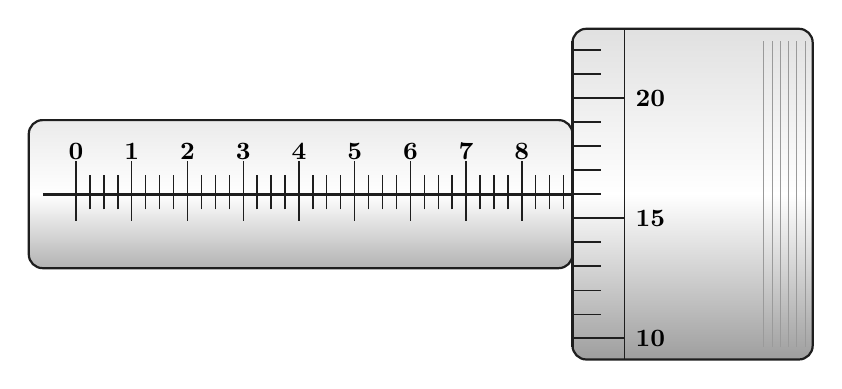
\begin{tikzpicture}[scale=1]
  \shade[rounded corners=5pt,top color=black!8,bottom color=black!30,middle color=white] (0,-0.94) rectangle (6.9055,0.94);
  \draw[scb,rounded corners=5pt] (0,-0.94) rectangle (6.9055,0.94);
  \draw[draw=figline,line width=1.1pt] (0.18,0) -- (6.9055,0);
  \draw[sc] (0.6,-0.336) -- (0.6,0.42);
  \node[lab,above] at (0.6,0.40) {0};
  \draw[sc] (0.7769,-0.192) -- (0.7769,0.24);
  \draw[sc] (0.9538,-0.192) -- (0.9538,0.24);
  \draw[sc] (1.1308,-0.192) -- (1.1308,0.24);
  \draw[sc] (1.3077,-0.336) -- (1.3077,0.42);
  \node[lab,above] at (1.3077,0.40) {1};
  \draw[sc] (1.4846,-0.192) -- (1.4846,0.24);
  \draw[sc] (1.6615,-0.192) -- (1.6615,0.24);
  \draw[sc] (1.8385,-0.192) -- (1.8385,0.24);
  \draw[sc] (2.0154,-0.336) -- (2.0154,0.42);
  \node[lab,above] at (2.0154,0.40) {2};
  \draw[sc] (2.1923,-0.192) -- (2.1923,0.24);
  \draw[sc] (2.3692,-0.192) -- (2.3692,0.24);
  \draw[sc] (2.5462,-0.192) -- (2.5462,0.24);
  \draw[sc] (2.7231,-0.336) -- (2.7231,0.42);
  \node[lab,above] at (2.7231,0.40) {3};
  \draw[sc] (2.9,-0.192) -- (2.9,0.24);
  \draw[sc] (3.0769,-0.192) -- (3.0769,0.24);
  \draw[sc] (3.2538,-0.192) -- (3.2538,0.24);
  \draw[sc] (3.4308,-0.336) -- (3.4308,0.42);
  \node[lab,above] at (3.4308,0.40) {4};
  \draw[sc] (3.6077,-0.192) -- (3.6077,0.24);
  \draw[sc] (3.7846,-0.192) -- (3.7846,0.24);
  \draw[sc] (3.9615,-0.192) -- (3.9615,0.24);
  \draw[sc] (4.1385,-0.336) -- (4.1385,0.42);
  \node[lab,above] at (4.1385,0.40) {5};
  \draw[sc] (4.3154,-0.192) -- (4.3154,0.24);
  \draw[sc] (4.4923,-0.192) -- (4.4923,0.24);
  \draw[sc] (4.6692,-0.192) -- (4.6692,0.24);
  \draw[sc] (4.8462,-0.336) -- (4.8462,0.42);
  \node[lab,above] at (4.8462,0.40) {6};
  \draw[sc] (5.0231,-0.192) -- (5.0231,0.24);
  \draw[sc] (5.2,-0.192) -- (5.2,0.24);
  \draw[sc] (5.3769,-0.192) -- (5.3769,0.24);
  \draw[sc] (5.5538,-0.336) -- (5.5538,0.42);
  \node[lab,above] at (5.5538,0.40) {7};
  \draw[sc] (5.7308,-0.192) -- (5.7308,0.24);
  \draw[sc] (5.9077,-0.192) -- (5.9077,0.24);
  \draw[sc] (6.0846,-0.192) -- (6.0846,0.24);
  \draw[sc] (6.2615,-0.336) -- (6.2615,0.42);
  \node[lab,above] at (6.2615,0.40) {8};
  \draw[sc] (6.4385,-0.192) -- (6.4385,0.24);
  \draw[sc] (6.6154,-0.192) -- (6.6154,0.24);
  \draw[sc] (6.7923,-0.192) -- (6.7923,0.24);
  \shade[rounded corners=5pt,top color=black!12,bottom color=black!38,middle color=white] (6.9055,-2.1) rectangle (9.9555,2.1);
  \draw[scb,rounded corners=5pt] (6.9055,-2.1) rectangle (9.9555,2.1);
  \draw[draw=figline,line width=1.0pt] (6.9055,-1.94) -- (6.9055,1.94);
  \draw[sc] (7.5655,-2.1) -- (7.5655,2.1);
  \draw[draw=figline!45,line width=0.4pt] (9.3355,-1.94) -- (9.3355,1.94);
  \draw[draw=figline!45,line width=0.4pt] (9.4405,-1.94) -- (9.4405,1.94);
  \draw[draw=figline!45,line width=0.4pt] (9.5455,-1.94) -- (9.5455,1.94);
  \draw[draw=figline!45,line width=0.4pt] (9.6505,-1.94) -- (9.6505,1.94);
  \draw[draw=figline!45,line width=0.4pt] (9.7555,-1.94) -- (9.7555,1.94);
  \draw[draw=figline!45,line width=0.4pt] (9.8605,-1.94) -- (9.8605,1.94);
  \draw[draw=figline,line width=0.9pt] (6.9055,-1.83) -- (7.5655,-1.83);
  \node[lab,right] at (7.6655,-1.83) {10};
  \draw[draw=figline,line width=0.5pt] (6.9055,-1.525) -- (7.2685,-1.525);
  \draw[draw=figline,line width=0.5pt] (6.9055,-1.22) -- (7.2685,-1.22);
  \draw[draw=figline,line width=0.5pt] (6.9055,-0.915) -- (7.2685,-0.915);
  \draw[draw=figline,line width=0.5pt] (6.9055,-0.61) -- (7.2685,-0.61);
  \draw[draw=figline,line width=0.9pt] (6.9055,-0.305) -- (7.5655,-0.305);
  \node[lab,right] at (7.6655,-0.305) {15};
  \draw[draw=figline,line width=0.5pt] (6.9055,0) -- (7.2685,0);
  \draw[draw=figline,line width=0.5pt] (6.9055,0.305) -- (7.2685,0.305);
  \draw[draw=figline,line width=0.5pt] (6.9055,0.61) -- (7.2685,0.61);
  \draw[draw=figline,line width=0.5pt] (6.9055,0.915) -- (7.2685,0.915);
  \draw[draw=figline,line width=0.9pt] (6.9055,1.22) -- (7.5655,1.22);
  \node[lab,right] at (7.6655,1.22) {20};
  \draw[draw=figline,line width=0.5pt] (6.9055,1.525) -- (7.2685,1.525);
  \draw[draw=figline,line width=0.5pt] (6.9055,1.83) -- (7.2685,1.83);
\end{tikzpicture}
}


\begin{document}

\begin{center}
  {\LARGE\bfseries EnergyTech}\\[2pt]
  {\Large Chapter 04}\\[6pt]
  Name: \rule{4.5cm}{0.4pt}\quad Group: \rule{3cm}{0.4pt}\quad SPSP ID: \rule{3.5cm}{0.4pt}
\end{center}

\begin{multicols}{2}
\raggedcolumns
% ---------------- Q1 ----------------
\begin{Qbox}{1}{4-1.1}
Determine the accuracy of the measurement; that is, give the number of significant digits for the measurement.\par\medskip $873{,}000$ lb
\begin{choices}
  \item 6
  \item 1
  \item 3
  \item 2
\end{choices}
\qrcode[height=2.2cm,hyperlink]{https://www.youtube.com/watch?v=FhLOHZ4jlP8}
\end{Qbox}

% ---------------- Q2 ----------------
\begin{Qbox}{2}{4-1.1}
Determine the accuracy of the measurement; that is, give the number of significant digits for the measurement.\par\medskip $504{,}9\overline{0}0$
\begin{choices}
  \item 5
  \item 6
  \item 8
  \item 4
\end{choices}
\qrcode[height=2.2cm,hyperlink]{https://www.youtube.com/watch?v=O2WRBUsIeZc}
\end{Qbox}

% ---------------- Q3 ----------------
\begin{Qbox}{3}{4-1.1}
Determine the accuracy of the measurement; that is, give the number of significant digits for the measurement.\par\medskip $0.00040$ g
\begin{choices}
  \item 2
  \item 4
  \item 3
  \item 1
\end{choices}
\qrcode[height=2.2cm,hyperlink]{https://www.youtube.com/watch?v=29VCgAWuS08}
\end{Qbox}

% ---------------- Q4 ----------------
\begin{Qbox}{4}{4-1.1}
Determine the accuracy of the measurement; that is, give the number of significant digits for the measurement.\par\medskip $0.0657000$ A
\begin{choices}
  \item 4
  \item 6
  \item 3
  \item 8
\end{choices}
\qrcode[height=2.2cm,hyperlink]{https://www.youtube.com/watch?v=gEq2wwiqNB8}
\end{Qbox}

% ---------------- Q5 ----------------
\begin{Qbox}{5}{4-1.1}
Determine the accuracy of the measurement; that is, give the number of significant digits for the measurement.\par\medskip $1{,}487$ m
\begin{choices}
  \item 5
  \item 3
  \item 6
  \item 4
\end{choices}
\qrcode[height=2.2cm,hyperlink]{https://www.youtube.com/watch?v=_FD3dS7Vg3U}
\end{Qbox}

% ---------------- Q6 ----------------
\begin{Qbox}{6}{4-1.1}
Determine the accuracy of the measurement; that is, give the number of significant digits for the measurement.\par\medskip $614{,}600$ g
\begin{choices}
  \item 4
  \item 6
  \item 3
  \item 5
\end{choices}
\qrcode[height=2.2cm,hyperlink]{https://www.youtube.com/watch?v=NZMZXixpuv4}
\end{Qbox}

% ---------------- Q7 ----------------
\begin{Qbox}{7}{4-2.1}
The measurement is 11.500 A. Find the precision.
\begin{choices}
  \item The precision of the measurement is 0.001 A.
  \item The precision of the measurement is 0.0001
  \item The precision of the measurement is 0.01 A
  \item The precision of the measurement is 0.1 A
\end{choices}
\qrcode[height=2.2cm,hyperlink]{https://www.youtube.com/watch?v=xKxx56lye3g}
\end{Qbox}

% ---------------- Q8 ----------------
\begin{Qbox}{8}{4-2.1}
The measurement is 17.00 cm. Find the precision.
\begin{choices}
  \item The precision is 0.1 cm
  \item The precision is 0.001 cm
  \item The precision is 0.01 cm
  \item The precision is 0.0001 cm.
\end{choices}
\qrcode[height=2.2cm,hyperlink]{https://www.youtube.com/watch?v=1JnWFd0IspY}
\end{Qbox}

% ---------------- Q9 ----------------
\begin{Qbox}{9}{4-2.1}
The measurement is 33.0000 in. Find the precision.
\begin{choices}
  \item The precision is 0.0001 in.
  \item The precision is 10 in
  \item The precision is 0.001 in
  \item The precision is 0.00001 in.
\end{choices}
\qrcode[height=2.2cm,hyperlink]{https://www.youtube.com/watch?v=kZ6FfJt_LTA}
\end{Qbox}

% ---------------- Q10 ----------------
\begin{Qbox}{10}{4-2.1}
The measurement is 344 km. Find the precision.
\begin{choices}
  \item The precision is 0.01 km.
  \item The precision is 10 km.
  \item The precision is 0.1 km.
  \item The precision is 1 km
\end{choices}
\qrcode[height=2.2cm,hyperlink]{https://www.youtube.com/watch?v=Uptz7jfWnVI}
\end{Qbox}

% ---------------- Q11 ----------------
\begin{Qbox}{11}{4-2.1}
The measurement is $49\overline{0}0$ km. Find the precision.
\begin{choices}
  \item The precision is 5 km
  \item The precision is 10 km.
  \item The precision is 50 km
  \item The precision is 100 km
\end{choices}
\qrcode[height=2.2cm,hyperlink]{https://www.youtube.com/watch?v=SE7YQtbcBeg}
\end{Qbox}

% ---------------- Q12 ----------------
\begin{Qbox}{12}{4-2.1}
The measurement is 40.60100 mi. Find the precision.
\begin{choices}
  \item The precision is 0.0001 mi.
  \item The precision is 0.01 mi
  \item The precision is 0.1 mi.
  \item The precision is 0.00001 mi
\end{choices}
\qrcode[height=2.2cm,hyperlink]{https://www.youtube.com/watch?v=cksn4vK3mhk}
\end{Qbox}

% ---------------- Q13 ----------------
\begin{Qbox}{13}{4-2.2}
The measurement is 13.5590 cm. Find the greatest possible error of the measurement.
\begin{choices}
  \item The greatest possible error is 0.00005 cm
  \item The greatest possible error is 0.0001 cm
  \item The greatest possible error is 0.005 cm
  \item The greatest possible error is 0.0005 cm
\end{choices}
\qrcode[height=2.2cm,hyperlink]{https://www.youtube.com/watch?v=L-TsjdvD7ZQ}
\end{Qbox}

% ---------------- Q14 ----------------
\begin{Qbox}{14}{4-2.2}
The measurement is 28.9100 m. Find the greatest possible error of the measurement.
\begin{choices}
  \item The greatest possible error is 0.005 m.
  \item The greatest possible error is 0.5 m
  \item The greatest possible error is 0.0005 m
  \item The greatest possible error is 0.00005 m
\end{choices}
\qrcode[height=2.2cm,hyperlink]{https://www.youtube.com/watch?v=QKBMWpAA95s}
\end{Qbox}

% ---------------- Q15 ----------------
\begin{Qbox}{15}{4-2.2}
The measurement is 15.300 m. Find the greatest possible error of the measurement.
\begin{choices}
  \item The greatest possible error is 5 m
  \item The greatest possible error is 0.0005 m.
  \item The greatest possible error is 0.5 m.
  \item The greatest possible error is 0.05 m
\end{choices}
\qrcode[height=2.2cm,hyperlink]{https://www.youtube.com/watch?v=7kzsFh5ax-8}
\end{Qbox}

% ---------------- Q16 ----------------
\begin{Qbox}{16}{4-2.1 / 4-2.2}
The measurement is $17\frac{12}{30}$ in. Find the precision and the greatest possible error of the measurement.
\begin{choices}
  \item Precision $=\dfrac{1}{30}$, greatest possible error $=\dfrac{1}{60}$
  \item Precision $=\dfrac{1}{60}$, greatest possible error $=\dfrac{1}{30}$
  \item Precision $=\dfrac{1}{30}$, greatest possible error $=\dfrac{1}{30}$
  \item Precision $=\dfrac{1}{60}$, greatest possible error $=\dfrac{1}{60}$
\end{choices}
\qrcode[height=2.2cm,hyperlink]{https://www.youtube.com/watch?v=FbGULnhUr58}
\end{Qbox}

% ---------------- Q17 ----------------
\begin{Qbox}{17}{4-2.1 / 4-2.2}
The measurement is $8\frac{23}{29}$ in. Find the precision and the greatest possible error of the measurement.
\begin{choices}
  \item Precision $=\dfrac{1}{58}$, greatest possible error $=\dfrac{1}{29}$
  \item Precision $=\dfrac{1}{29}$, greatest possible error $=\dfrac{1}{58}$
  \item Precision $=\dfrac{1}{29}$, greatest possible error $=\dfrac{1}{29}$
  \item Precision $=\dfrac{1}{58}$, greatest possible error $=\dfrac{1}{58}$
\end{choices}
\qrcode[height=2.2cm,hyperlink]{https://www.youtube.com/watch?v=8v8T6GLrV7M}
\end{Qbox}

% ---------------- Q18 ----------------
\begin{Qbox}{18}{4-3.1}
In the given Vernier Caliper, part J is \ldots
\incfig{210}{fig_caliper.png}
\begin{choices}
  \item Depth gauge
  \item Jaws
  \item Beam
  \item Small jaws
\end{choices}
\qrcode[height=2.2cm,hyperlink]{https://www.youtube.com/watch?v=CKAhOUBv_Ck}
\end{Qbox}

% ---------------- Q19 ----------------
\begin{Qbox}{19}{4-3.1}
In the given Vernier Caliper, part H is \ldots
\incfig{210}{fig_caliper.png}
\begin{choices}
  \item Metric Vernier scale
  \item U.S. Fixed scale
  \item Metric Fixed scale
  \item U.S. Vernier scale
\end{choices}
\qrcode[height=2.2cm,hyperlink]{https://www.youtube.com/watch?v=eydw_enMeQk}
\end{Qbox}

% ---------------- Q20 ----------------
\begin{Qbox}{20}{4-3.1}
Read the measurement in millimeter shown on the vernier caliper.
\figbox{\figQBZ}
\begin{choices}
  \item 25.60 mm
  \item 52.60 mm
  \item 2.069 mm
  \item 2.096 mm
\end{choices}
\qrcode[height=2.2cm,hyperlink]{https://www.youtube.com/watch?v=m5Lp71cWcFE}
\end{Qbox}

% ---------------- Q21 ----------------
\begin{Qbox}{21}{4-3.2}
Read the measurement in millimeter shown on the vernier caliper.
\figbox{\figQBA}
\begin{choices}
  \item 110.50 mm
  \item 115.90 mm
  \item 120.56 mm
  \item 4.562 mm
\end{choices}
\qrcode[height=2.2cm,hyperlink]{https://www.youtube.com/watch?v=xVg0hxrQ4Jg}
\end{Qbox}

% ---------------- Q22 ----------------
\begin{Qbox}{22}{4-3.3}
Read the measurement in inch shown on the vernier caliper.
\figbox{\figQBB}
\begin{choices}
  \item 2.36 in
  \item 2.236 in
  \item 0.236 in
  \item 56.75 in
\end{choices}
\qrcode[height=2.2cm,hyperlink]{https://www.youtube.com/watch?v=wcmLZgkqi3M}
\end{Qbox}

% ---------------- Q23 ----------------
\begin{Qbox}{23}{4-3.3}
Read the measurement in inch shown on the vernier caliper.
\figbox{\figQBC}
\begin{choices}
  \item 1.417 in
  \item 0.417 in
  \item 0.714 in
  \item 1.714 in
\end{choices}
\qrcode[height=2.2cm,hyperlink]{https://www.youtube.com/watch?v=bXo3POT01eE}
\end{Qbox}

% ---------------- Q24 ----------------
\begin{Qbox}{24}{4-4.1}
In the given Micrometer Caliper, part K is
\incfig{200}{fig_micrometer.png}
\begin{choices}
  \item Ratchet
  \item Thimble
  \item Spindle
  \item Anvil
\end{choices}
\qrcode[height=2.2cm,hyperlink]{https://www.youtube.com/watch?v=0XkBVkZvfvA}
\end{Qbox}

% ---------------- Q25 ----------------
\begin{Qbox}{25}{4-4.1}
In the given Micrometer Caliper, part J is
\incfig{200}{fig_micrometer.png}
\begin{choices}
  \item Ratchet
  \item Thimble
  \item Spindle
  \item Anvil
\end{choices}
\qrcode[height=2.2cm,hyperlink]{https://www.youtube.com/watch?v=89Bz6HZpME8}
\end{Qbox}

% ---------------- Q26 ----------------
\begin{Qbox}{26}{4-4.2}
Read the measurement shown on the metric micrometer.
\figbox{\figQBF}
\begin{choices}
  \item 3.13 mm
  \item 3.15 mm
  \item 3.14 mm
  \item 30.14 mm
\end{choices}
\qrcode[height=2.2cm,hyperlink]{https://www.youtube.com/watch?v=n0lpdXKX8NA}
\end{Qbox}

% ---------------- Q27 ----------------
\begin{Qbox}{27}{4-4.2}
Read the measurement shown on the metric micrometer.
\figbox{\figQBG}
\begin{choices}
  \item 87.5 mm
  \item 8.25 mm
  \item 8.75 mm
  \item 8.50 mm
\end{choices}
\qrcode[height=2.2cm,hyperlink]{https://www.youtube.com/watch?v=MplthM6FZQU}
\end{Qbox}

% ---------------- Q28 ----------------
\begin{Qbox}{28}{4-4.4}
Read the measurement shown on the U.S. micrometer.
\figbox{\figQBH}
\begin{choices}
  \item 0.398 in
  \item 3.098 in
  \item 0.400 in
  \item 0.423 in
\end{choices}
\qrcode[height=2.2cm,hyperlink]{https://www.youtube.com/watch?v=tTfhEPs7AG4}
\end{Qbox}

% ---------------- Q29 ----------------
\begin{Qbox}{29}{4-4.3}
Read the measurement shown on the U.S. micrometer.
\figbox{\figQBI}
\begin{choices}
  \item 8.750 in
  \item 8.910 in
  \item 0.875 in
  \item 0.891 in
\end{choices}
\qrcode[height=2.2cm,hyperlink]{https://www.youtube.com/watch?v=BSleiTcnV88}
\end{Qbox}

% ---------------- Q30 ----------------
\begin{Qbox}{30}{4-5.1}
Find the measurement that is the most accurate.
\begin{choices}
  \item 100 ft
  \item 8,200 ft
  \item 536 ft
  \item 820 ft
\end{choices}
\qrcode[height=2.2cm,hyperlink]{https://www.youtube.com/watch?v=wFtUtuKgrnI}
\end{Qbox}

% ---------------- Q31 ----------------
\begin{Qbox}{31}{4-5.1}
Find the measurement that is the most accurate.
\begin{choices}
  \item 945 ft
  \item 600 ft
  \item 110 ft
  \item 1,100 ft
\end{choices}
\qrcode[height=2.2cm,hyperlink]{https://www.youtube.com/watch?v=fi2FP7z8XXk}
\end{Qbox}

% ---------------- Q32 ----------------
\begin{Qbox}{32}{4-5.1}
Find the measurement that is the most accurate.
\begin{choices}
  \item 1,800 ft
  \item 180 ft
  \item 400 ft
  \item 921 ft
\end{choices}
\qrcode[height=2.2cm,hyperlink]{https://www.youtube.com/watch?v=S8T8OfIpWdU}
\end{Qbox}

% ---------------- Q33 ----------------
\begin{Qbox}{33}{4-5.1}
Find the measurement that is the most accurate.
\begin{choices}
  \item 5000 ft
  \item 0.00580 ft
  \item 0.8900 ft
  \item 2300 ft
\end{choices}
\qrcode[height=2.2cm,hyperlink]{https://www.youtube.com/watch?v=kmIhRWkySiY}
\end{Qbox}

% ---------------- Q34 ----------------
\begin{Qbox}{34}{4-5.1}
Find the measurement that is the least accurate.
\begin{choices}
  \item 0.00020 in
  \item 3000 in
  \item 15.8000 in
  \item 0.000320 in
\end{choices}
\qrcode[height=2.2cm,hyperlink]{https://www.youtube.com/watch?v=i50ZER16Vic}
\end{Qbox}

% ---------------- Q35 ----------------
\begin{Qbox}{35}{4-5.1}
Find the measurement that is the least accurate.
\begin{choices}
  \item 1250000 m
  \item 150000 m
  \item 0.00520 m
  \item 36100 m
\end{choices}
\qrcode[height=2.2cm,hyperlink]{https://www.youtube.com/watch?v=M7AB8u72_8k}
\end{Qbox}

% ---------------- Q36 ----------------
\begin{Qbox}{36}{4-5.1}
Find the measurement that is the least accurate.
\begin{choices}
  \item 23000 in
  \item 0.000230 in
  \item 52.0000 in
  \item 1000 in
\end{choices}
\qrcode[height=2.2cm,hyperlink]{https://www.youtube.com/watch?v=d32PX6zaUhM}
\end{Qbox}

% ---------------- Q37 ----------------
\begin{Qbox}{37}{4-5.1}
Find the measurement that is the most accurate.
\begin{choices}
  \item 0.093 A
  \item 0.00030 A
  \item 0.0660 A
  \item 0.092 A
\end{choices}
\qrcode[height=2.2cm,hyperlink]{https://www.youtube.com/watch?v=kfDJ24QBcuI}
\end{Qbox}

% ---------------- Q38 ----------------
\begin{Qbox}{38}{4-5.1}
Find the measurement that is the least accurate.
\begin{choices}
  \item 2,600,000 V
  \item 21,000 V
  \item 33,000 V
  \item 20,000 V
\end{choices}
\qrcode[height=2.2cm,hyperlink]{https://www.youtube.com/watch?v=CdvPb7S0h9Y}
\end{Qbox}

% ---------------- Q39 ----------------
\begin{Qbox}{39}{4-5.1}
Find the measurement that is the least accurate.
\begin{choices}
  \item 26,000 V
  \item 4,600,000 V
  \item 8,100 V
  \item 80,000 V
\end{choices}
\qrcode[height=2.2cm,hyperlink]{https://www.youtube.com/watch?v=mdd_74Yj1iA}
\end{Qbox}

% ---------------- Q40 ----------------
\begin{Qbox}{40}{4-5.1}
Find the measurement that is the least accurate.
\begin{choices}
  \item 23.00 V
  \item 13,500 V
  \item 0.00820 V
  \item 0.0015 V
\end{choices}
\qrcode[height=2.2cm,hyperlink]{https://www.youtube.com/watch?v=L0pMHrjqsEg}
\end{Qbox}

% ---------------- Q41 ----------------
\begin{Qbox}{41}{4-5.1}
Find the measurement that is the least accurate.
\begin{choices}
  \item 5.380 ft
  \item 0.2500 ft
  \item 52,000 ft
  \item 5.20000 ft
\end{choices}
\qrcode[height=2.2cm,hyperlink]{https://www.youtube.com/watch?v=nQ0DitEi1Ps}
\end{Qbox}

% ---------------- Q42 ----------------
\begin{Qbox}{42}{4-5.1}
Find the measurement that is the least accurate.
\begin{choices}
  \item 770 ft
  \item 501 ft
  \item 600 ft
  \item 591 ft
\end{choices}
\qrcode[height=2.2cm,hyperlink]{https://www.youtube.com/watch?v=Y1cHxGjrkjU}
\end{Qbox}

% ---------------- Q43 ----------------
\begin{Qbox}{43}{4-5.1}
Find the measurement that is the least accurate.
\begin{choices}
  \item 200 ft
  \item 946 ft
  \item 890 ft
  \item 906 ft
\end{choices}
\qrcode[height=2.2cm,hyperlink]{https://www.youtube.com/watch?v=eBSkNlhA6Wc}
\end{Qbox}

% ---------------- Q44 ----------------
\begin{Qbox}{44}{4-5.1}
Find the measurement that is the least accurate.
\begin{choices}
  \item 406 ft
  \item 426 ft
  \item 520 ft
  \item 300 ft
\end{choices}
\qrcode[height=2.2cm,hyperlink]{https://www.youtube.com/watch?v=toC9PYl0yHk}
\end{Qbox}

% ---------------- Q45 ----------------
\begin{Qbox}{45}{4-5.1}
Use the rules of measurements to evaluate.\par\medskip $(5{,}300\ \text{cm})(39.00\ \text{cm})$
\begin{choices}
  \item $206{,}700$ cm$^2$
  \item $210{,}000$ cm$^2$
  \item $200{,}000$ cm$^2$
  \item $206{,}000$ cm$^2$
\end{choices}
\qrcode[height=2.2cm,hyperlink]{https://www.youtube.com/watch?v=_Xjo5E_pcYo}
\end{Qbox}

% ---------------- Q46 ----------------
\begin{Qbox}{46}{4-6.1}
Use the rules of measurements to evaluate.\par\medskip $(2{,}400\ \text{m})(80\ \text{m})(1320\ \text{m})$
\begin{choices}
  \item $253{,}440{,}000$ m$^3$
  \item $253{,}400{,}000$ m$^3$
  \item $253{,}000{,}000$ m$^3$
  \item $300{,}000{,}000$ m$^3$
\end{choices}
\qrcode[height=2.2cm,hyperlink]{https://www.youtube.com/watch?v=vd7Sg-5mZc0}
\end{Qbox}

% ---------------- Q47 ----------------
\begin{Qbox}{47}{4-6.1}
Use the rules of measurements to evaluate.\par\medskip $52{,}800$ V $\div\ 3.4$ A
\begin{choices}
  \item $15{,}529$ V/A
  \item $15{,}530$ V/A
  \item $15{,}500$ V/A
  \item $16{,}000$ V/A
\end{choices}
\qrcode[height=2.2cm,hyperlink]{https://www.youtube.com/watch?v=rLAH-4JSDRo}
\end{Qbox}

% ---------------- Q48 ----------------
\begin{Qbox}{48}{4-6.1}
Use the rules of measurements to evaluate.\[ \frac{(3250\ m)(2.8\ L)}{6.0\ s} \]
\begin{choices}
  \item $1{,}517\ mL/s$
  \item $2{,}000\ mL/s$
  \item $1.500\ mL/s$
  \item $1{,}500\ mL/s$
\end{choices}
\qrcode[height=2.2cm,hyperlink]{https://www.youtube.com/watch?v=rGtejzjn64U}
\end{Qbox}

% ---------------- Q49 ----------------
\begin{Qbox}{49}{4-6.1}
Find the area of a rectangle 2.20 cm by 52.0 cm. $(A=l\cdot w)$ (Use the rules for working with measurements).
\begin{choices}
  \item $114$ cm$^2$
  \item $110$ cm$^2$
  \item $100$ cm$^2$
  \item $114.4$ cm$^2$
\end{choices}
\qrcode[height=2.2cm,hyperlink]{https://www.youtube.com/watch?v=OVOHkqfkrEI}
\end{Qbox}

% ---------------- Q50 ----------------
\begin{Qbox}{50}{4-6.1}
Find the volume of a rectangular solid when $l=2.80$ ft, $w=8.0$ ft, and $h=62.20$ ft.\par\medskip $V=lwh$, where $l$ length, $w$ width, and $h$ height.\par\medskip (Use the rules for working with measurements)
\begin{choices}
  \item $1{,}393.28$ ft$^3$
  \item $1{,}390$ ft$^3$
  \item $1{,}400$ ft$^3$
  \item $1{,}393$ ft$^3$
\end{choices}
\qrcode[height=2.2cm,hyperlink]{https://www.youtube.com/watch?v=6P8cDZvSm3M}
\end{Qbox}

\end{multicols}
\end{document}
